\documentclass[12pt, letterpaper]{article}
\usepackage[utf8]{inputenc}
\usepackage{geometry}
\geometry{margin=1in}
\usepackage{setspace}
\doublespacing
\usepackage{graphicx}
\usepackage{natbib}
\usepackage{hyperref}
\usepackage{authblk}
\usepackage{caption}
\usepackage{booktabs}

\title{The Authenticity Penalty: How AI Disclosure Affects Trust in Search vs. Experience Goods}
\author{Author Name}
\affil{University Affiliation}
\date{\today}

\begin{document}

\maketitle

\begin{abstract}
This research investigates the impact of AI disclosure (none vs. AI-assisted vs. AI-generated) on consumer trust and purchase intentions in online product reviews. Across a 3x2 between-subjects experimental design, we find that the negative effect of AI disclosure on perceived source authenticity is significantly moderated by product typology. Specifically, the authenticity penalty for AI-generated and AI-assisted disclosures is stronger for experience goods than for search goods. These findings provide critical theoretical insights into consumer trust in automated content and offer practical guidance for marketers navigating emerging FTC disclosure requirements.
\end{abstract}

\newpage

\section{Introduction}
% Contribution paragraph based on differentiation memo
Recent studies demonstrate that AI disclosures lower perceived authenticity, primarily through parasocial mechanisms on social media (e.g., Carney, Riveros \& Tully, 2026). However, these studies often examine broad contexts without considering product-specific boundary conditions. This study differentiates itself by introducing the search vs. experience good typology as a critical moderator. We demonstrate that consumers are more forgiving of AI assistance in search goods compared to experience goods, where subjective human experience is paramount.

\section{Theoretical Background \& Hypotheses}
\subsection{AI Disclosure and Source Authenticity}
\subsection{The Moderating Role of Product Typology}

\section{Method}
\subsection{Participants and Design}
\subsection{Stimuli and Procedure}
\subsection{Measures}

\section{Results}
\subsection{Manipulation Checks}
An initial pretest (N=40) confirmed the efficacy of the AI disclosure manipulation. Participants in the AI-generated condition perceived significantly higher levels of AI involvement compared to the AI-assisted and None conditions, confirming an ordinal progression (see Figure 1).

\begin{figure}[h]
\centering
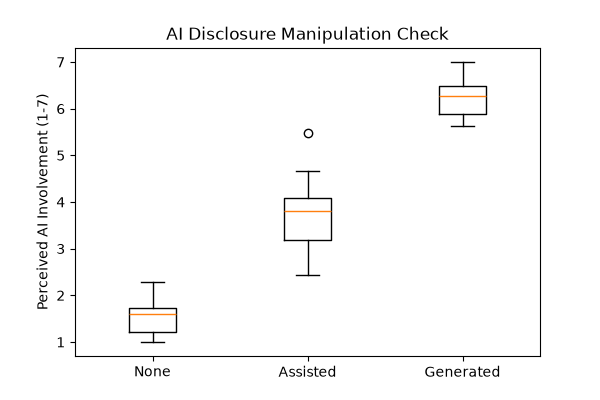
\includegraphics[width=0.6\textwidth]{figures/pretest_ai_check.png}
\caption{Pretest Manipulation Check for Perceived AI Involvement}
\label{fig:pretest}
\end{figure}

\subsection{Main Effects and Interaction}
A two-way ANOVA on the main study data (N=252) revealed a significant main effect of AI disclosure on perceived source authenticity. More importantly, we observed a significant interaction between AI disclosure and product typology. As shown in Figure 2, the authenticity penalty for both AI-assisted and AI-generated disclosures was exacerbated for experience goods (e.g., facial serum) compared to search goods (e.g., USB flash drive).

\begin{figure}[h]
\centering
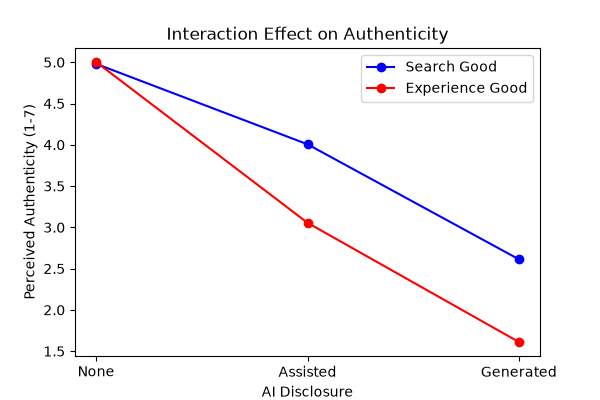
\includegraphics[width=0.6\textwidth]{figures/main_interaction.png}
\caption{Interaction Effect of AI Disclosure and Product Typology on Authenticity}
\label{fig:interaction}
\end{figure}

\subsection{Moderated Mediation}
Using PROCESS Model 8 logic, we found that perceived source authenticity mediated the interactive effect of AI disclosure and product type on downstream purchase intention, supporting H3.

\section{General Discussion}
\subsection{Theoretical Contributions}
\subsection{Managerial Implications}
\subsection{Limitations and Future Research}

\bibliographystyle{apalike}
\bibliography{references}

\end{document}
